\chapter{Les factures}
Les factures sont comme les devis une des fonctionnalités les plus importantes de l'application. De propriétés semblable, il est aussi possible de créer plusieurs factures pour un projet.
\section{Liste des factures\index{Facture!Liste}}
Pour afficher les factures d'un projet il faut, à partir du panneau contenant la liste des projets d'un client, faire un double clic sur le projet en question. La liste affichée contient les factures et les devis du projet sélectionné auparavant. C'est la même liste qui est affichée si l'on cherche à afficher les devis.

\section{Ajouter une facture\index{Facture!Ajouter}}
Pour ajouter une facture, il est nécessaire de sélectionner un client dans le panneau central (si l'on est dans la liste des projets ou des factures, la nouvelle facture sera automatiquement ajouté à ce client). Une fois le client selectionné on crée une nouvelle facture en cliquant sur le bouton << Nouvelle facture >> de la barre d'outils ou via le menu << Client $\rightarrow$ Nouvelle facture >>. 
\begin{figure}[H]
	\centering
	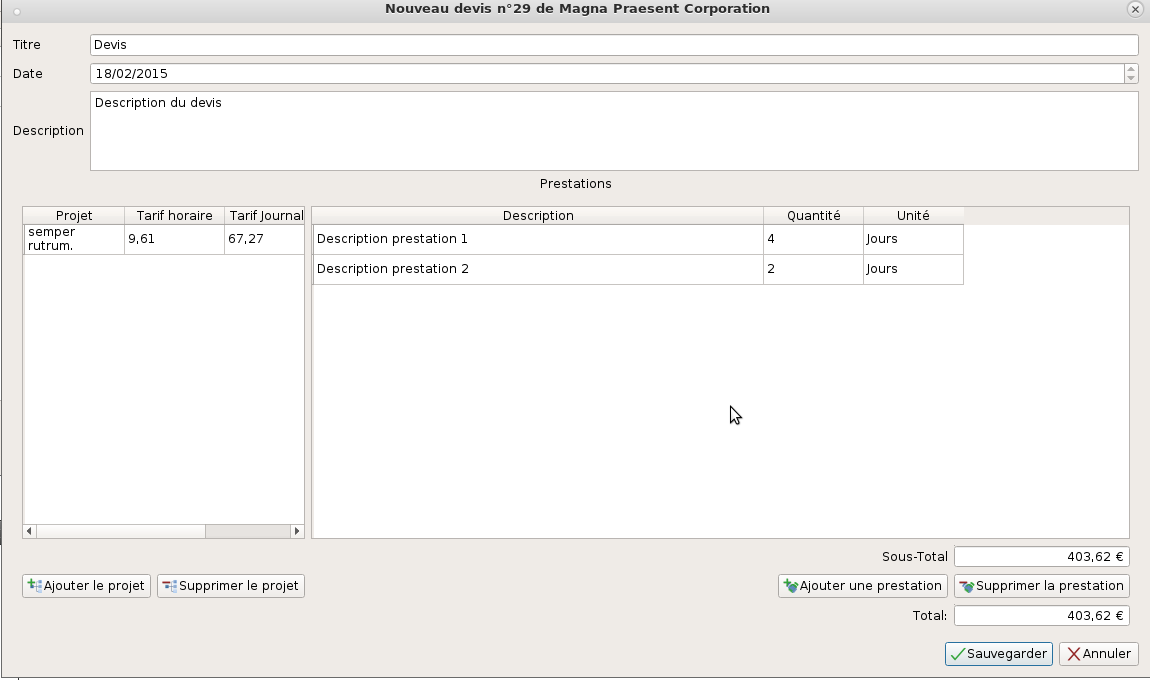
\includegraphics[width=7cm]{screens/creerDevis.png}
	\caption{Créer une nouvelle facture à un projet client}
\end{figure}
Une facture possède un titre à afficher, une date (celle du jour de création du projet), une description et la liste des prestations qui lui sont associées. 
\section{Les Prestations\index{Facture!Prestation}}
La liste des prestations sont affichées dans la fenêtre d'ajout d'une facture\index{Facture!Ajouter}. Une prestation peut être ajoutée, respectivement supprimée en utilisant les boutons << Ajouter une prestation >> et << Supprimer une prestation >>. Dans le cas d'un ajout, une nouvelle ligne est ajoutée au tableau des prestations. Cette ligne indique à quel projet est associé la prestation, une description de la prestation et le nombre d'heures que l'on va y consacrer. 